\chapter{Measurements of Charge Transfer Efficiency in the SNIFS Detectors}
\label{chap:cte}

\section{Introduction}
Charge-coupled devices (CCDs) are ubiquitous in optical and infrared astronomy. Incident photons generate electrons in the bulk silicon of the CCD, and these photoelectrons are then collected by a grid of pixels arranged on a series of parallel readout registers. By manipulating the voltages of the gates that separate the pixels of these registers, we can shuffle the collected charge row-by-row into a additional register, known as the serial register. Similar voltage manipulations of the serial register gates produce an output signal that can be amplified and digitized. The charge shuffling procedure alternates between the parallel and serial registers until all pixels have been read out, and an image can then be reconstructed from the resulting signal.

Ideally, 100\% of the charge in each pixel would be transferred to the next pixel at each readout step. However, traps in the silicon lattice of the CCD can capture charge only to release it at a later time. The trapped and released charge leads to smearing of point sources along the direction of charge transfer and impedes our ability to get accurate photon counts. The magnitude of this effect is quantified by the charge transfer efficiency (CTE) of the CCD, defined as the fraction of charge that survives each pixel transfer. Because most of the CCDs used in astronomical applications make many transfers in each image (as they have thousands of pixels in each register), the CTE must be very close to unity, with typical values being around $1-10^{-6}$. Additionally, because a larger number of transfers results in a higher likelihood of encountering more traps, pixels that are further from the readout register are more affected by charge trapping. This effect is especially problematic for spectroscopic instruments since the increased smearing with distance to the amplifier can lead to effects like uneven broadening of spectral features.

In this work, we quantify the charge transfer efficiency of the CCDs in all channels (photometric, and blue and red spectroscopic) of the SuperNova Integral Field Spectrograph (SNIFS). SNIFS is the main instrument used by the Nearby Supernova Factory \citep[SNfactory, ]{aldering_overview_2002} project, which was designed to spectrophotometrically observe Type Ia supernovae at redshifts around $z=0.07$. The instrument is a two-channel integral field spectrograph, mounted on the University of Hawai`i 2.2m telescope on Maunakea. A dichroic mirror splits the light into the red and blue spectroscopic channels, covering the wavelength ranges of 3200–5200\,\AA{} and 5100–10,000\,\AA, respectively. Two microlens arrays split the 6$''$~x~6$''$ field of view into 225 samples of 0.4$''$~x~0.4$''$. The light eventually reaches the detectors. For the blue channel, the detector is a 2048~x~4096 pixel thin CCD, while for the red channel the detector is a 2048~x~4096 pixel deep-depletion CCD. In addition to the spectroscopic channels, there are also the guiding and photometric channel of the instrument. This channel is located at the focus of the telescope, where we have two deep-depleted CCD detectors -- one used for guiding the telescope, and the other used in conjunction with various filters for photometric observations. Each of the CCD detectors in the SNIFS instrument have 2 amplifiers, which we label A and B in the spectroscopic channels. The two detectors of the guiding and photometric channels are treated as a single detector in the read out software, so we label the amplifiers of the first detector A and B, and call the amplifiers of the second detector C and D. 

We use two techniques to measure the CTE in all of these detectors. The initial characterization of the SNIFS CCDs is done by first exposing them to a Fe$^{55}$ x-ray source in order to generate single-pixel events with a known energy spectrum and then measuring the photoelectron loss directly. Later, we perform a similar analysis using cosmic ray events extracted from the dark frames taken during each SNIFS observing run. These in-situ measurements of the CTE allow us to track changes in the efficiency over time.

\section{Initial Characterization with \texorpdfstring{Fe$^{55}$}{Fe-55} X-rays}
A standard method for measuring CTE involves exposing the CCD to photons with a known energy spectrum \citep{janesick_scientific_2001}. X-ray sources are high enough energy to generate many electron-hole pairs in a small volume in the CCD, typically resulting in a detectable event in the image that takes up a single pixel. Because we know the energy spectrum of these events, we can easily calculate the expected distribution of the number of electrons in these single-pixel events. By plotting the amount of charge measured in each event as a function of the row number, we can quantify the extent of charge trapping by measuring the decrease in charge with distance from the amplifier.

A common source for these characterizations is Fe$^{55}$, which produces strong lines from $K_\alpha$ and $K_\beta$ emission at 5.9 keV and 6.2 keV. These emission lines corresponding to photoelectron signals in the CCD of 1620 $\textrm{e}^-$ and 1778 $\textrm{e}^-$, respectively, as the amount of energy necessary to produce an electron-hole pair in silicon is approximately 3.65 eV in the regime where the photon energy is greater than approximately 10 eV.

Each of the SNIFS CCDs were exposed to a Fe$^{55}$ source a number of times, producing images like the one shown in Figure \ref{fig:example_xray_image}. Using \verb|sep| \citep{barbary_sep_2015}, a Python implementation of the commonly-used \verb|SExtractor| package \citep{bertin_sextractor_1996}, we selected all events in the resulting images that had signal levels $>5\sigma$ above the background signal level determined with a filter size of 32 x 32 pixels. We then fit the histogram of digitized counts in these extracted events, binned into 10 count bins, to a simple double-Gaussian model of the Fe$^{55}$ spectrum:
\begin{equation}
    s = A_\alpha \exp\left(-\frac{(f-1620/g)^2}{2\sigma_\alpha^2}\right) + A_\beta \exp\left(-\frac{(f-1778/g)^2}{2\sigma_\beta^2}\right).
\end{equation}
This fit is done in order to measure the gain, $g$, of the CCD amplifier, allowing us to convert from ADU counts to electrons. The relative fraction of events from the $K_\alpha$ and $K_\beta$ emission ($A_\alpha/A_\beta$), as well as the widths of the emission lines ($\sigma_\alpha$ and $\sigma_\beta$) are allowed to float, and we treat these parameters as nuisance parameters in the fit to obtain the gain.

\begin{figure}
    \centering
    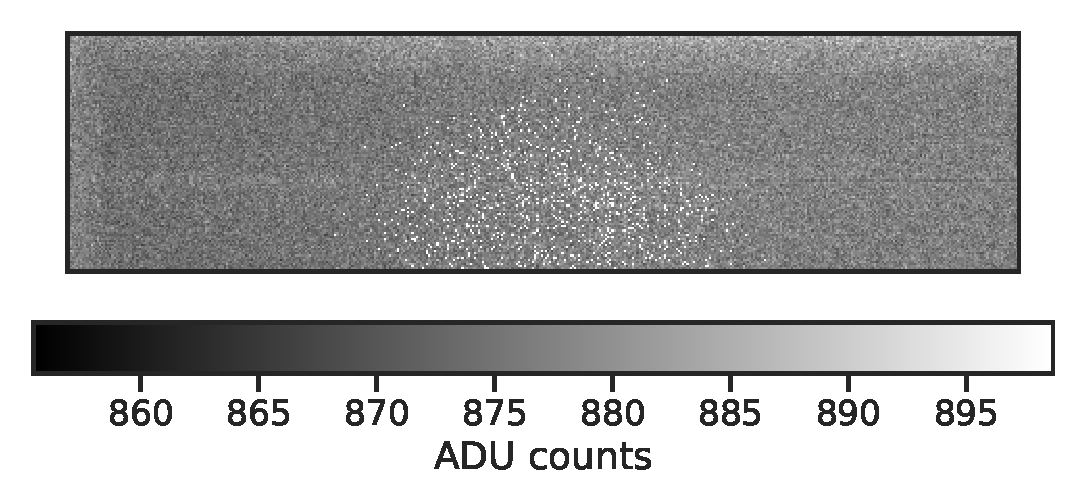
\includegraphics[width=0.9\textwidth]{figures/cte/example_xray_image.pdf}
    \caption{Example X-ray image for a single amplifier.}
    \label{fig:example_xray_image}
\end{figure}

\begin{figure}
    \centering
    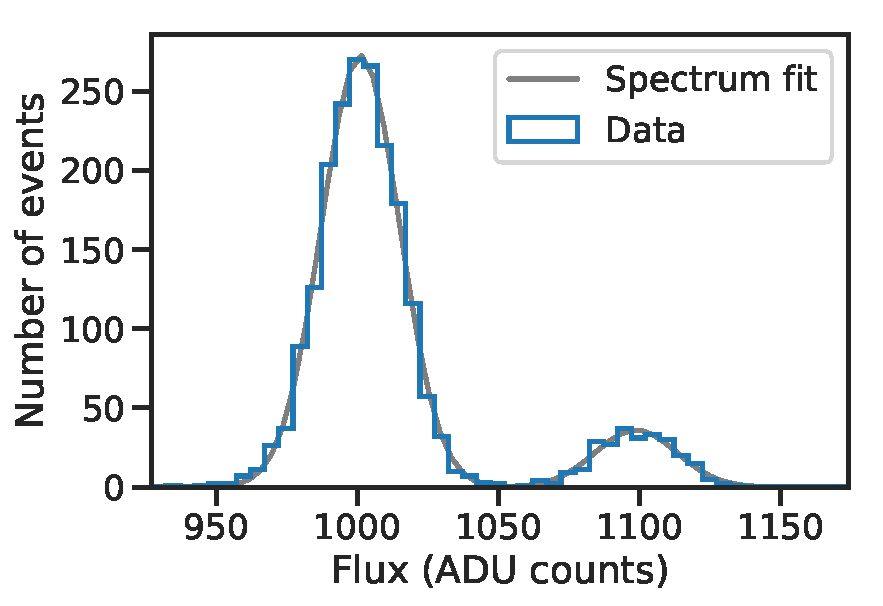
\includegraphics{figures/cte/spectrum_fit.pdf}
    \caption{Example spectrum of the Fe$^{55}$ X-rays events extracted from a single amplifier frame along with the best-fit model. The results of this fit are used to determine the amplifier gain from each frame.}
    \label{fig:xray_spectrum}
\end{figure}

Using these gain measurements to convert the ADU counts to the number of electrons $N_{e^-}$, we are able to combine the events from several images per channel (22 for the blue channel, 26 for the red channel, and 8 for the photometric channel). We select the events that correspond to $K_\alpha$ emission with a simple cut, choosing events with $1550 < N_{e^-} < 1700$. We then plot the flux for each event as a function of distance from the amplifier, shown in Figure \ref{fig:cte_xray} for the parallel registers and Figure \ref{fig:cte_xray_serial} for the serial register. The slope of the best-fit line (in units of $e^-$ per transfer), divided by the expected number of electrons (1620), gives us our measurement of the charge transfer \textit{in}efficiency, the number of electrons lost per transfer ($\textrm{CTI}=1-\textrm{CTE}$). The resulting measurements of the charge transfer inefficiency are shown as labels in Figs. \ref{fig:cte_xray} and \ref{fig:cte_xray_serial}, as well as in Table \ref{tab:cte_xray}. All of the parallel values are on the order of $10^{-6}$, i.e. about one electron in every million is lost in each transfer. The serial CTI values are slightly higher; this is acceptable because there are fewer transfers that need to be done in the serial direction.

\begin{figure}[htbp]
    \centering
    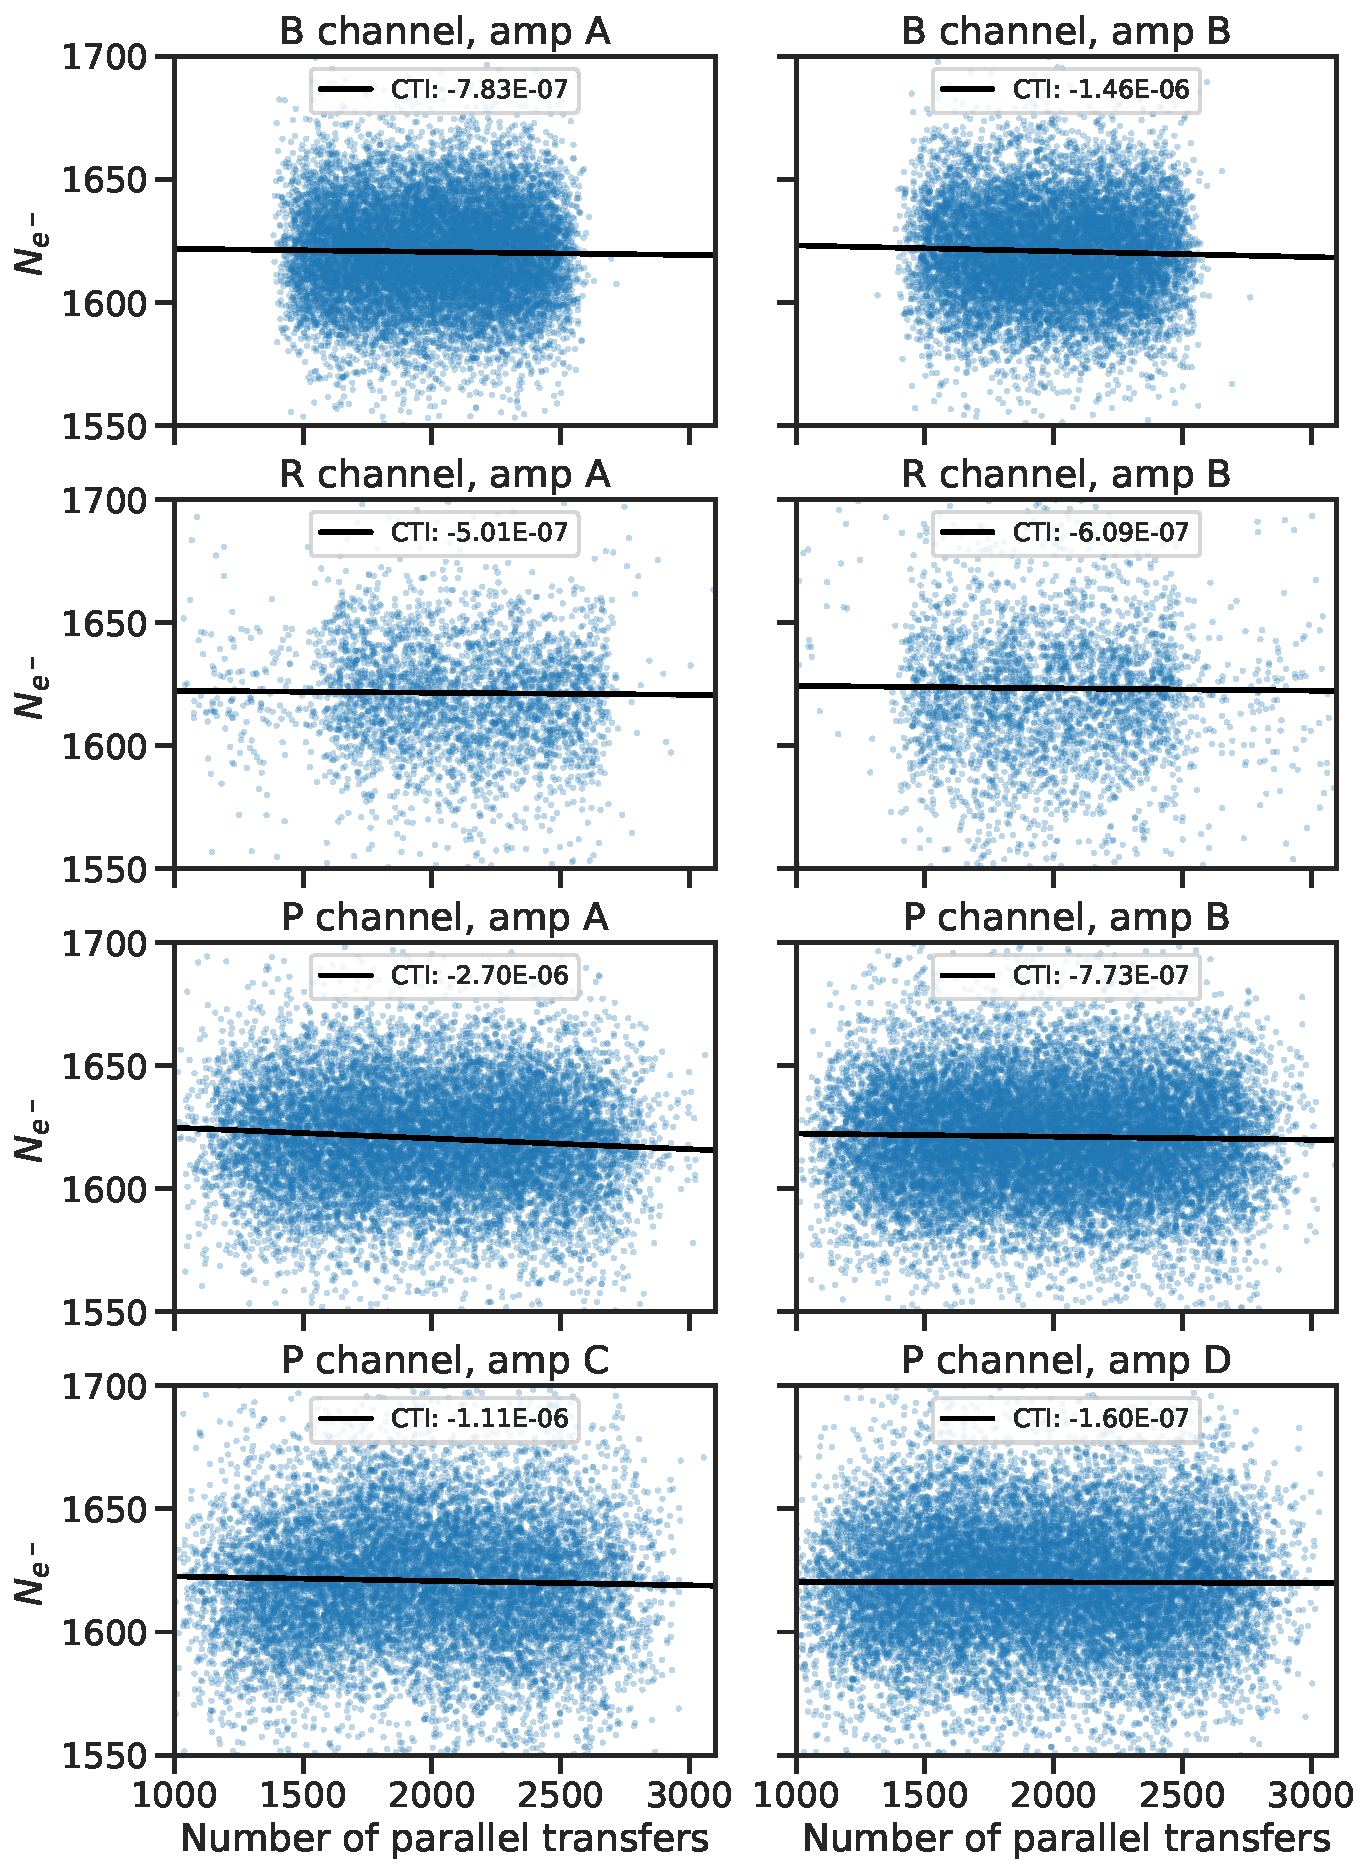
\includegraphics[width=0.8\textwidth]{figures/cte/xray_cte_parallel.pdf}
    \caption{The number of electrons in extracted Fe$^{55}$ X-ray events as a function of y-location on the CCD for each camera amplifier (equivalent to number of transfers in the parallel direction). The slope of the best-fit line divided by the expected number of electrons gives us an estimate of the charge transfer inefficiency in the parallel registers.}
    \label{fig:cte_xray}
\end{figure}

\begin{figure}[htbp]
    \centering
    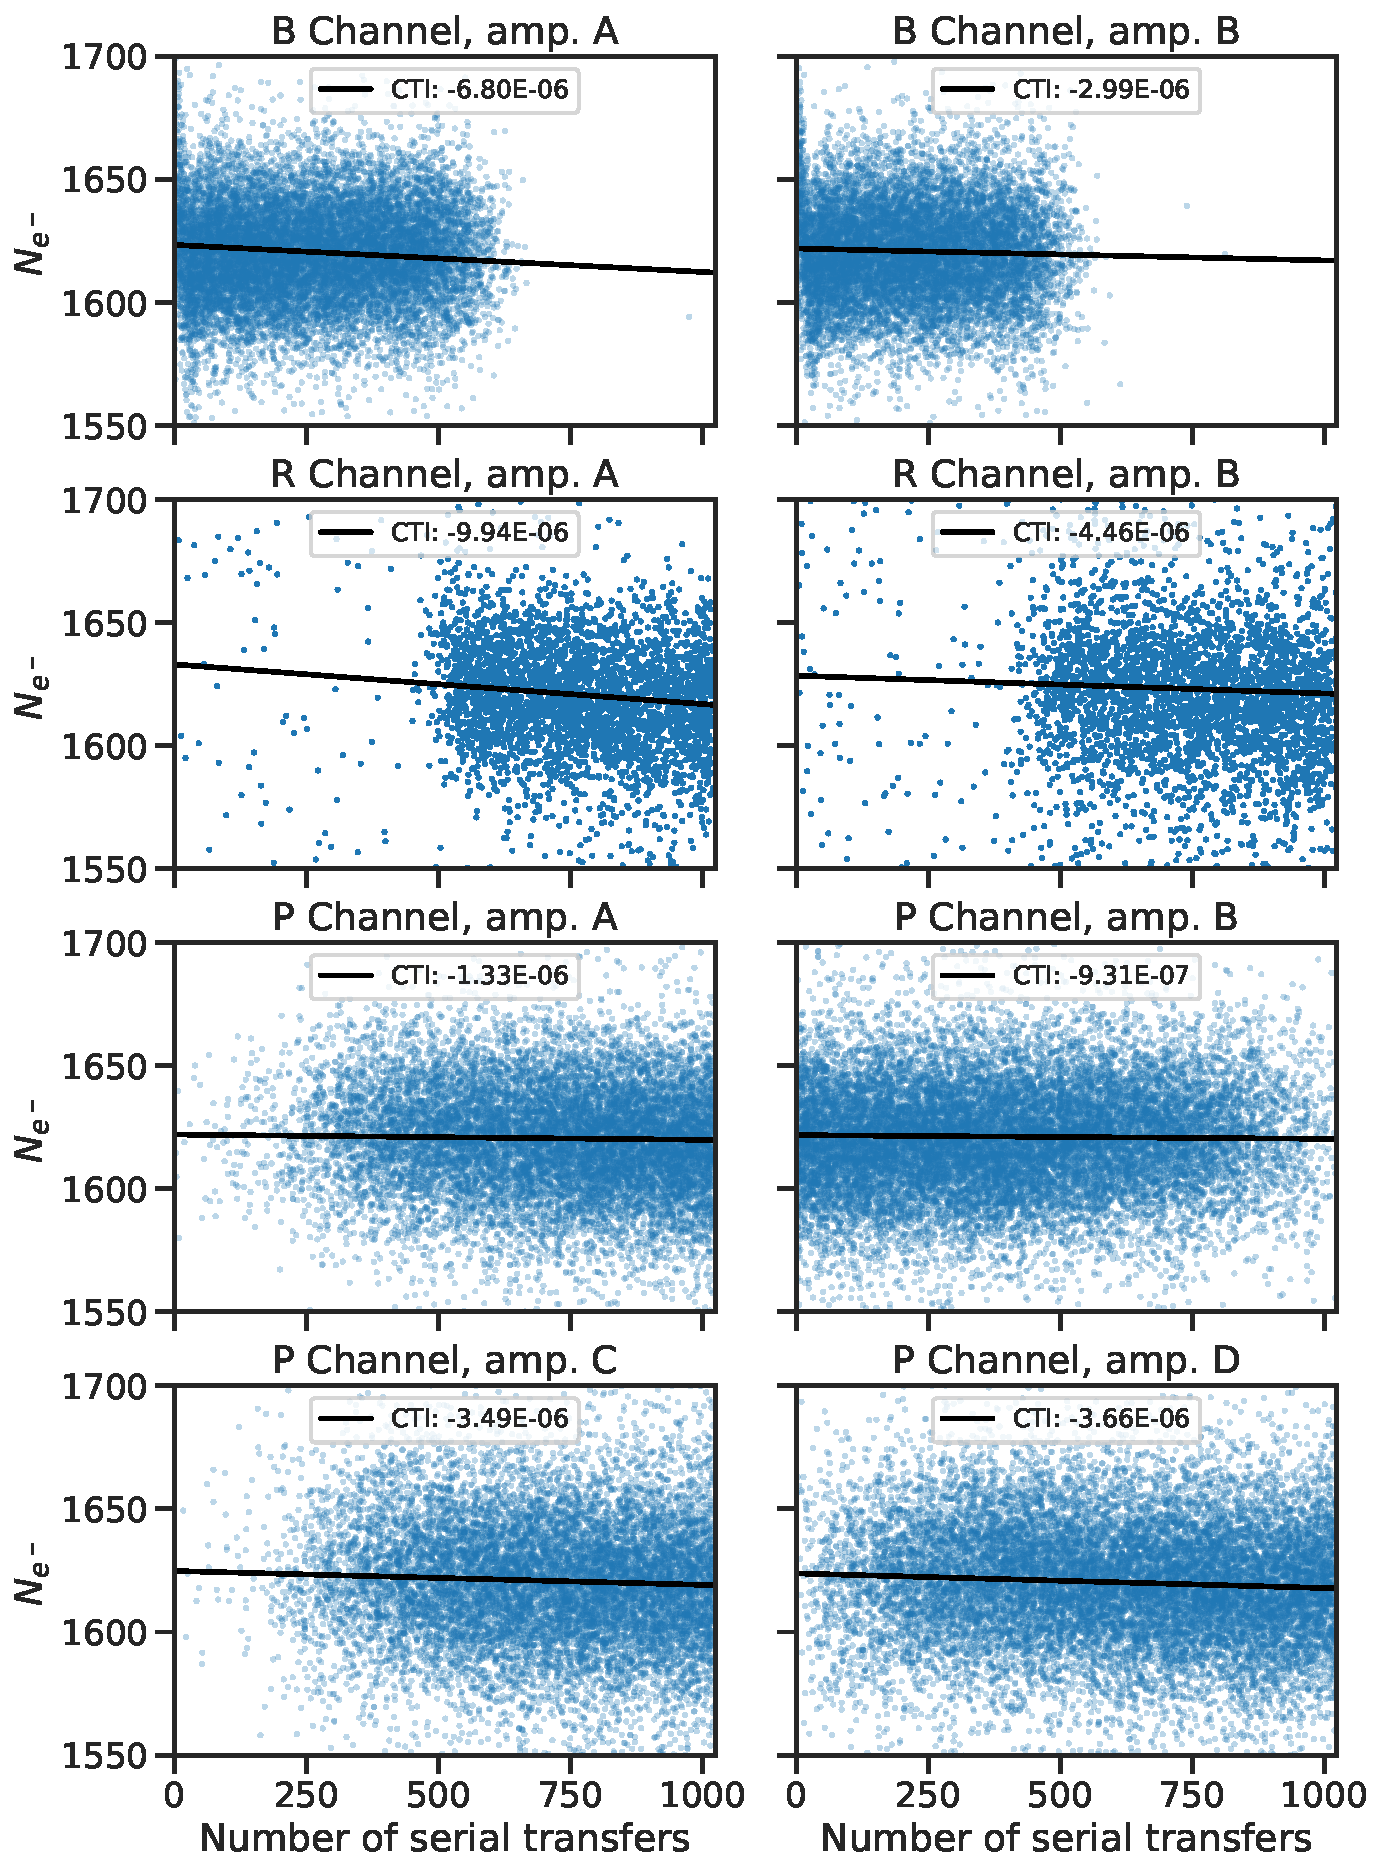
\includegraphics[width=0.8\textwidth]{figures/cte/xray_cte_serial.pdf}
    \caption{Same as Figure \ref{fig:cte_xray}, but for the x-location of events. The best-fit lines are used to estimate the charge transfer inefficiency in the serial registers.}
    \label{fig:cte_xray_serial}
\end{figure}

\begin{table}[htbp]
    \centering
    \begin{tabular}{cccccc}\toprule
        Camera & Amp. & Parallel CTI & Serial CTI & Number of images & Number of events \\\midrule
        B & A &0.783 $\;\pm\;$ 0.015 & 6.80 $\;\pm\;$ 0.03 & 22 & 15,925 \\
        B & B &1.455 $\;\pm\;$ 0.017 & 2.99 $\;\pm\;$ 0.03 &  & 13,113 \\\midrule
        R & A &0.501 $\;\pm\;$ 0.013 & 9.94 $\;\pm\;$ 0.04 & 26 & 4,071 \\
        R & B &0.609 $\;\pm\;$ 0.011 & 4.46 $\;\pm\;$ 0.03 &  & 4,415 \\\midrule
        P & A &2.696 $\;\pm\;$ 0.010 & 1.33 $\;\pm\;$ 0.02 & 8 & 15,308 \\
        P & B &0.773 $\;\pm\;$ 0.008 & 0.93 $\;\pm\;$ 0.01 &  & 21,010 \\
        P & C &1.111 $\;\pm\;$ 0.009 & 3.49 $\;\pm\;$ 0.02 &  & 14,498 \\
        P & D &0.160 $\;\pm\;$ 0.008 & 3.66 $\;\pm\;$ 0.01 &  & 19,041 \\
    \end{tabular}
    \caption{Charge transfer inefficiency results from Fe$^{55}$ X-ray characterization. All values are in units of $10^{-6}$.}
    \label{tab:cte_xray}
\end{table}

\section{Cosmic Ray Measurement}
The X-ray measurement allows for a precise determination of the CTE when we have physical access to the detector. However, we'd like to be able to track changes in the CTE with time in situ in order to quantify any degradation over the lifetime of the instrument. We can get such a measurement by making use of the cosmic ray hits found in the dark frames taken as part of normal observing procedure and measuring the average smearing of these hits due to charge transfer inefficiency, similar to the methodology presented in \cite{riess_time_1999}.

Cosmic rays create small (approximate 6-7 pixels) events in CCD images. The shape of each individual event is driven by the incidence angle of the cosmic ray and charge diffusion (i.e. bleeding between pixels because of the structure of the CCD), but also by the CTI smearing effect. The first two effects are statistically symmetric about the highest pixel, so in principle we should be able to subtract the symmetric portions of the cosmic ray events, leaving only the asymmetric CTI trails.

We proceed very similarly to \cite{riess_time_1999}. We restrict ourselves to dark frame images that had an exposure time of 1 hour in order to have a high enough count of cosmic ray events in the image. For each of these dark frames, we use \verb|sep| to find cosmic ray hits, defined as the objects detected at $>1.5\sigma$ over the background level, with a measured ellipticity $< 0.2$ and no flags raised by \verb|sep|. The ellipticity cut serves to remove extremely oblique incidence events or coincident events from our sample, as both types of event add excess noise to the measurement. Example hits that pass these cuts are shown in Figure \ref{fig:example_hits}. Additionally, in order to avoid the noise potentially introduced by hits landing in the CTI trails of other nearby hits (see e.g. the bottom right example in Figure \ref{fig:example_hits}), we remove from our sample all pairs of events that are within 10 pixels of one another.

\begin{figure}
    \centering
    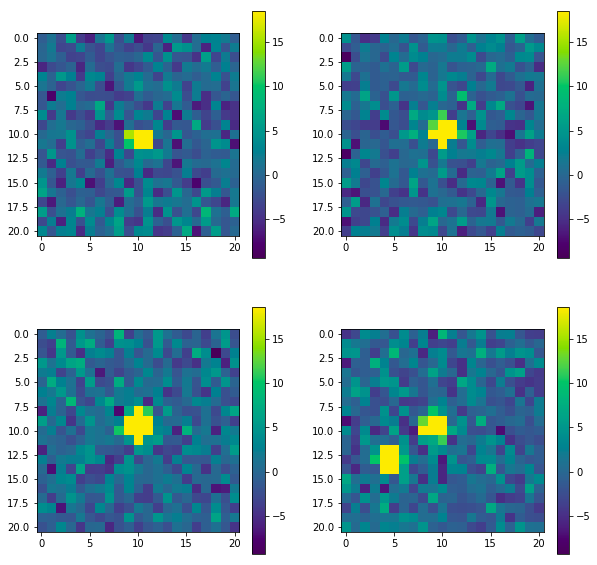
\includegraphics[width=0.9\textwidth]{figures/cte/example_hits.png}
    \caption{Example identified cosmic ray hits passing our ellipticity cut. The two neighboring hits seen in the bottom right example would be removed from the final sample because they are too close to each other. This culling removes some of the noise from our final signal.}
    \label{fig:example_hits}
\end{figure}

For each selected cosmic ray event, we subtract the value of the pixels further from the readout amplifier from the pixels closer to the readout amplifier in both the parallel and serial direction. We then calculate the fraction of charge that is left in the trail by summing the number of excess counts in the 5 trailing pixels and dividing that sum by the number of counts in the peak of the event. On average, this gives us an estimate of the fraction of charge lost to trapping. 
    
To boost our statistics, we aggregate all of these measured charge loss fractions on a nightly basis. The individual values of the charge loss fraction are shown in blue in Figs. \ref{fig:cte_single_night} and \ref{fig:cte_single_night_serial}. These measurements are extremely noisy, so to reduce the noise, we group them in 16 bins along the direction of interest and take the median and normalized median absolute deviation (NMAD) of all of the measurements in each bin. These median values are shown in red in Figs. \ref{fig:cte_single_night} and \ref{fig:cte_single_night_serial}, as well as in Figure \ref{fig:cte_single_night_medians} and \ref{fig:cte_single_night_serial_medians} in more detail. Finally, we fit a line to these median values weighted by the NMAD in each bin. As before, the slope of the line gives us a measure of the charge transfer inefficiency.

\begin{figure}
    \centering
    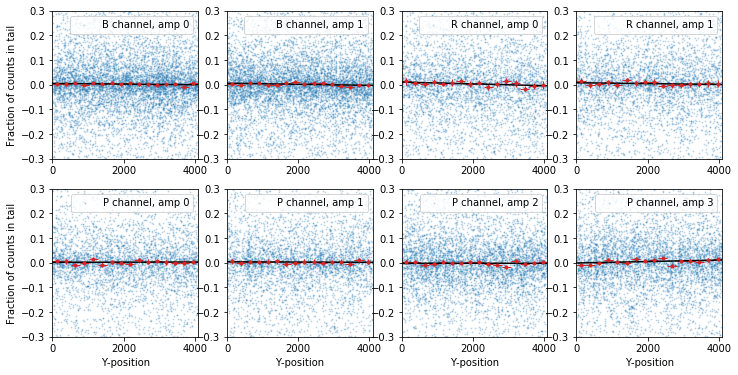
\includegraphics[width=0.9\textwidth]{figures/cte/single_night_example_parallel.png}
    \caption{Example measurement of CTI in the parallel register from cosmic ray trails from a single night. All blue dots represent a single cosmic ray hit. The red points show the median fraction of counts in the peak of the hits that end up in the trails in each y-position bin. The best-fit line is also shown. The slope of this line gives us the CTI.}
    \label{fig:cte_single_night}
\end{figure}

\begin{figure}
    \centering
    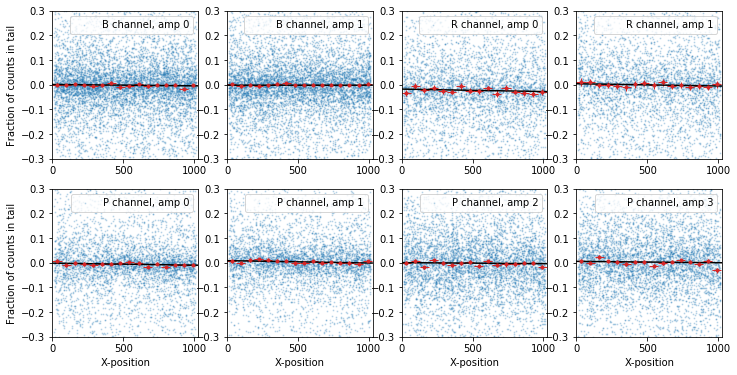
\includegraphics[width=0.9\textwidth]{figures/cte/single_night_example_serial.png}
    \caption{Same as Figure \ref{fig:cte_single_night} but in the serial direction.}
    \label{fig:cte_single_night_serial}
\end{figure}

\begin{figure}
    \centering
    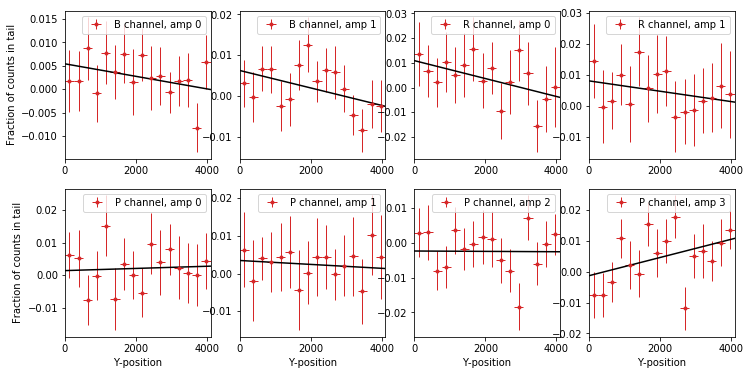
\includegraphics[width=0.9\textwidth]{figures/cte/single_night_example_parallel_medians.png}
    \caption{Same as Figure \ref{fig:cte_single_night} but zoomed to show the median values and their associated uncertainties.}
    \label{fig:cte_single_night_medians}
\end{figure}

\begin{figure}
    \centering
    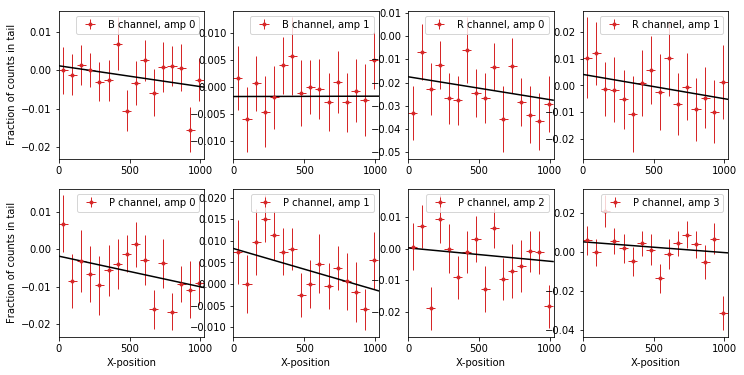
\includegraphics[width=0.9\textwidth]{figures/cte/single_night_example_serial_medians.png}
    \caption{Same as Figure \ref{fig:cte_single_night_medians} but in the serial direction.}
    \label{fig:cte_single_night_serial_medians}
\end{figure}

We made these measurements for every night's dark frames in order to check for time dependence. In Figure \ref{fig:time_variation} we show the CTI in the parallel and serial registers as a function of time for each amplifier. Figure \ref{fig:time_variation_binned} shows the same data aggregated by year. We find that there is very little evidence of significant degradation over time. Indeed, linear fits to each of these yearly aggregated data sets have slopes consistent with zero. Finally, the median CTI measured in each amplifier using cosmic rays in dark frames are all summarized in Table \ref{tab:cte_darks}.

The values are roughly consistent with what was found in the X-ray measurements, as all CTI values are still on the order of $10^6$, with the serial registers having higher CTI than the parallel registers. There are a number of potential reasons for the remaining differences between the measurements. One possible source of the difference in these two measurements could be that the X-ray measurement photons were focused on the center of each CCD, whereas the cosmic ray measurements are dispersed over the full chip. As a result, there were portions of the CCD that no X-ray photoelectrons passed through, so the effect of charge traps in these regions would be neglected by these measurements. There were also some challenges in identifying true single-pixel X-ray events, particularly in the deep-depleted CCDs (red spectroscopic and photometric channels), where the discrepancies are largest). The X-ray photoelectrons can be deposited deeper in the silicon of these CCDs, creating multi-pixel halos rather than the expected single-pixel events. Some of these fractional events may happen to be detected over our background threshold and thus be counted as a single-pixel event. This effect could also be exacerbated by event-crowding, where several fractional events are combined because they occur in neighboring pixels, and the combined events are misidentified as a single event. Overall, while the cosmic ray measurements are much noisier, as the measurement of the fraction of charge lost is much more subject to noise, these aggregated measurements are more reliable and more useful for tracking CCD performance over time. 

\begin{figure}
    \centering
    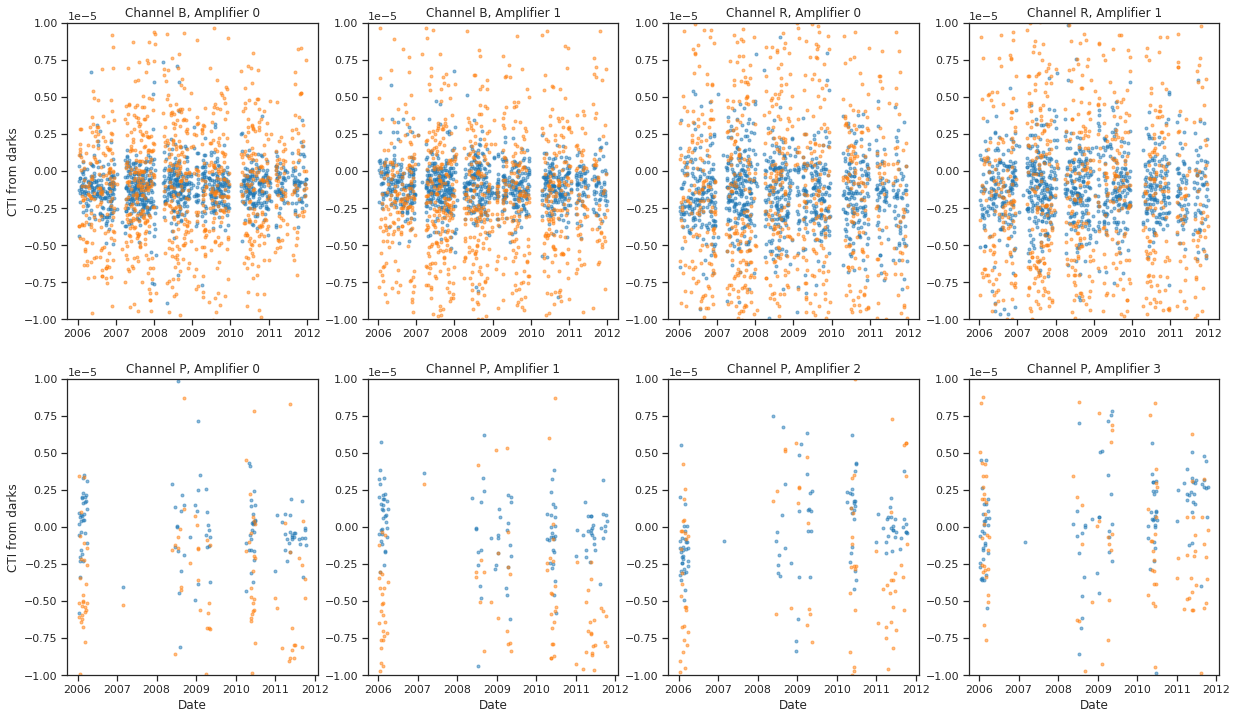
\includegraphics[width=0.9\textwidth]{figures/cte/time_variation.png}
    \caption{A search for potential time variation in the charge transfer efficiency of each of the spectroscopic cameras. CTI measurements in the parallel direction are shown in blue and those in the serial direction are shown in orange.}
    \label{fig:time_variation}
\end{figure}

\begin{figure}
    \centering
    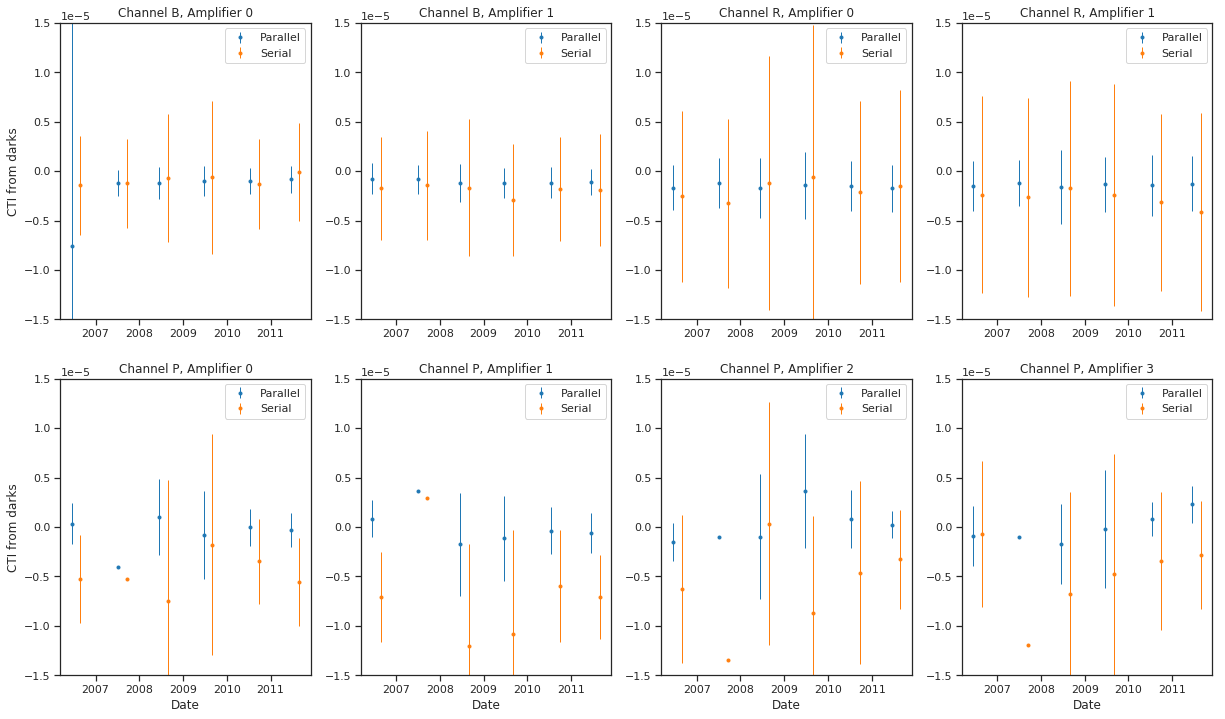
\includegraphics[width=0.9\textwidth]{figures/cte/time_variation_by_year.png}
    \caption{Same as Fig \ref{fig:time_variation} but aggregated by year.}
    \label{fig:time_variation_binned}
\end{figure}

\begin{table}[htbp]
    \centering
    \begin{tabular}{cccc}\toprule
        Camera & Amplifier & Median Parallel CTI  & Median Serial CTI \\ \midrule
        B & A &   1.08 $\pm$ 0.04  &  0.96 $\pm$ 0.13 \\
          & B &   0.97 $\pm$ 0.04  &  2.02 $\pm$ 0.13 \\\midrule
        R & A &   1.49 $\pm$ 0.07  &  2.4  $\pm$ 0.2 \\
          & B &   1.24 $\pm$ 0.07  &  2.3  $\pm$ 0.2 \\\midrule
        P & A &   0.19 $\pm$ 0.18  &  5.1  $\pm$ 0.5 \\
          & B &   0.18 $\pm$ 0.19  &  7.0  $\pm$ 0.4 \\
          & C &   0.3  $\pm$ 0.2   &  5.4  $\pm$ 0.7 \\
          & D &   0.5  $\pm$ 0.2   &  1.9  $\pm$ 0.5 \\\midrule
    \end{tabular}
    \caption{CTI measurements over time from all dark frames collected from 2006 to 2012. All values are in units of $10^{-6}$.}
    \label{tab:cte_darks}
\end{table}

\section{Conclusion}
We have presented two separate measurements of the charge transfer efficiency of the SNIFS CCD, first with an X-ray source in the laboratory, and later in situ using cosmic ray events in dark frames to measure the average fraction of charge lost in readout. The latter measurement is noisier, but allowed us to track evolution of CTE over time. We see no evidence of such evolution. Our measurements are roughly consistent with one another, to within an order of magnitude, and both measurements show that the charge transfer inefficiency is sufficiently low for the detectors' use in spectroscopy. The code used in this work is publicly available at \url{https://www.github.com/sam-dixon/cte}.


